\section{Pattern Matching}

\subsection{Brute-Force Algorithmus}
\subsubsection{Definition}
\begin{itemize}
    \item vergleicht das Pattern P mit dem Text T für jede mögliche Position von P relativ zu T, bis entweder
    \begin{itemize}
        \item eine Übereinstimmung gefunden
        \item alle möglichen Platzierungen des Patterns ausprobiert
    \end{itemize}
\end{itemize}
\subsubsection{Laufzeit}
\begin{itemize}
    \item benötigt O(nm) Zeit
    \item Worst Case:
    \begin{itemize}
        \item T = aaa...ah (Text)
        \item P = aaah (Pattern)
        \item Treten  in  Bild-Analysen  und  DNA  Sequenzenauf, Text eher nicht
    \end{itemize}
\end{itemize}
\subsubsection{Algorithmus}
\begin{lstlisting}
Algorithm BruteForceMatch(T, P)
    Input Text T der Laenge n und Pattern P der Laenge m
    Output Startindex eines Substrings von T, welcher mit P uebereinstimmt, oder -1 falls keiner gefunden wurde

    for i <- 0 to n-m { testen der i-ten Verschiebung des Patterns }
        k <- 0
        while j < m && T [i + j] = P[j]
            j <- j+1 if j = m
        return i {match bei i}
    return -1 {kein match}
\end{lstlisting}


\subsection{Boyer-Moore Algorithmus}
\subsubsection{Definition}
Basiert auf zwei Heuristiken:
    \begin{itemize}
        \item \textbf{Looking-Glass:} vergleiche P mit einer Subsequenz von T. Starte dabei am Ende des Patterns
        \item \textbf{Character-Jump:} falls bei T[i] = c keine Übereinstimmung
        \begin{itemize}
            \item falls P das Zeichen c enthält, verschiebe P bis das letzte Auftreten von c in P mit T[i] übereinstimmt.
            \item sonst, verschiebe P bis P[0] mit T[i + 1] übereinstimmt
        \end{itemize}
    \end{itemize}
\vspace{-8pt}
\begin{center}
    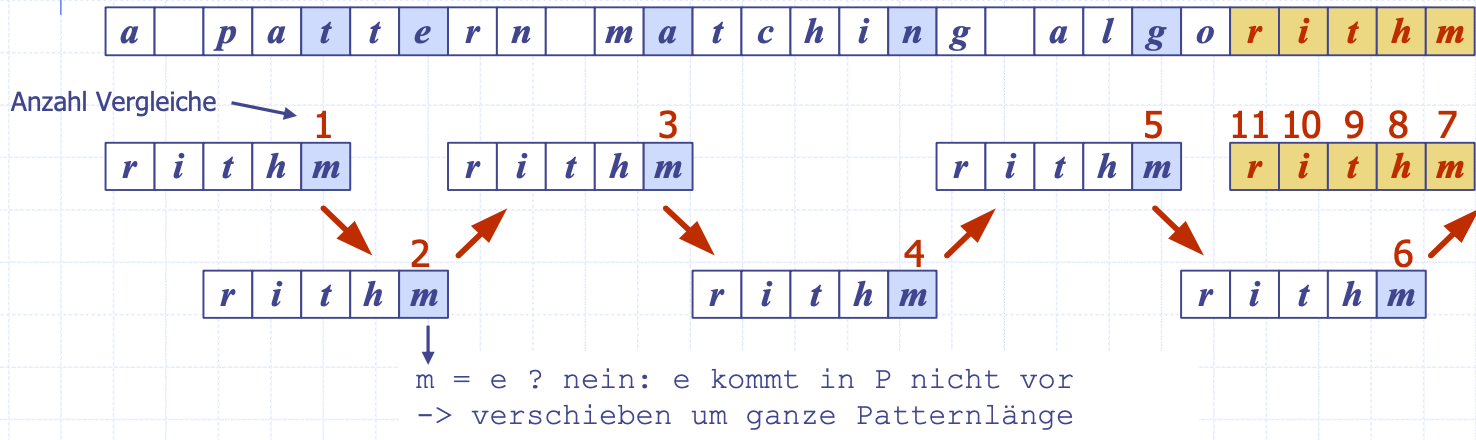
\includegraphics[scale=.25]{graphic/08 PatternMatching/Boyer-Moore def.png}
\end{center}
\vspace{-8pt}
\subsubsection{Laufzeit}
\begin{itemize}
    \item benötigt O(n * m + s)
    \item Worst Case:
    \begin{itemize}
        \item T=aaa...a
        \item P=baaa
    \end{itemize}
    \item Worst-Case kommt vor allem bei Bild- und DNA- Sequenzen vor und ist bei Text unwahrscheinlich
    \item ist signifikant schneller als der Brute-Force Algorithmus (angewandt auf Textanalysen)
\end{itemize}
\subsubsection{Algorithmus}
\begin{enumerate}
    \item Ist bereits das erste verglichene Textsymbol ein Symbol, das im Muster überhaupt nicht vorkommt, so kann das Muster um m Positionen hinter dieses Symbol weitergeschoben werden
    \item Falls eine Ungleichheit auftritt, das fehlerhafte Zeichen aber an anderer Stelle im Muster vorkommt, dann kann das Muster nur so weit geschoben werden, bis dieses Vorkommen ("die andere Stelle") auf das Textsymbol ausgerichtet ist
    \item Ergibt es eine negative Verschiebung, schiebe stattdessen um 1
\end{enumerate}
\subsection{Last-Occurrence Funktion}
Boyer-Moore's Algorithmus analysiert zuerst das Pattern P und das Alphabet $\Sigma$, um die last-occurrence Funktion L aufzubauen.\\
Diese bildet $\Sigma$ auf Integers ab, wobei L(c) wie folgt definiert ist:
\begin{itemize}
    \item $ L: \Sigma \rightarrow lN_0 \cup {-1}$
    \item $L: c \rightarrow L(c) =max_i {i|P[i]=c}$ falls c in P vorkommt, sonst -1
\end{itemize}
\begin{center}
    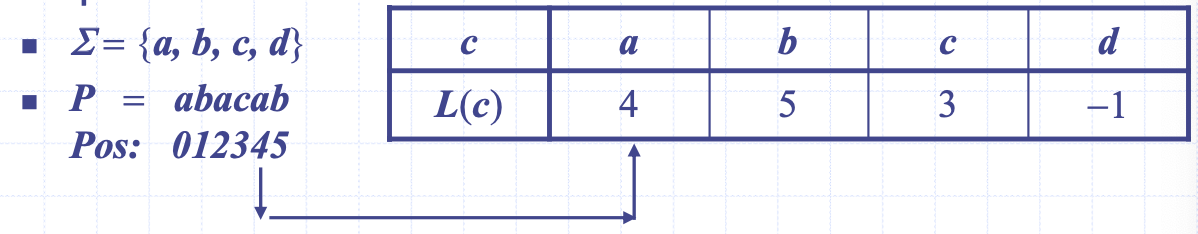
\includegraphics[scale=.28]{graphic/08 PatternMatching/Last-Occurrence.png}
\end{center}
\begin{itemize}
    \item Die Funktion L(c) lässt sich darstellen als ein Array, dessen Indices durch numerische Werte des Alphabets gegeben sind.
    \item Die Funktion lässt sich in O(m + s) berechnen, wobei m die Länge von P und s die Anzahl Zeichen in $\Sigma$ ist.
\end{itemize}
\subsubsection{Berechnung der Verschiebung}

\begin{itemize}
    \item Fall 1: Zeichen T[i] kommt im Pattern vor (last(T[i]> -1))
    \begin{itemize}
        \item Verschieben bis zum letzten Auftreten des Zeichens im Pattern
        \item Berechnung: i = i + m - (last(T[i]) + 1)
    \end{itemize}
    \item Fall 2: Zeichen kommt im Pattern vor, ist aber bereits vorhanden
    \begin{itemize}
        \item Pattern wird nach eine Stelle nach vorne verschoben
        \item i = i + m - j
    \end{itemize}
\end{itemize}

\paragraph{Boyer-Moore Algorithmus}

\textbf{1. "Last-Occurrence" - Funktion L(c) bestimmen}\\

\textbf{Spalte c:} Alle Buchstaben, die im Text vorkommen\\
\textbf{Spalte L(c):} falls im Pattern: letzte Position\\ 
\textbf{Spalte L(c):} falls nicht im Pattern: -1 \\

\textbf{2. Vergleichen}\\
Immer der hinterste Buchstaben des Patterns wird mit Text verglichen!\\

\textbf{3. Missmatch}\\
\begin{tabular}[]{p{2cm} p{3.8cm}}
    Buchstabe im Text & Ausrichten auf letztes Element\\
                      & bei negativer Verschiebung $\rightarrow$ 1 nach rechts\\
    \hline
    Buchstabe kommt \underline{nicht} im Text vor & Verschieben um ganze Patternlänge
\end{tabular}

\vfill
$ $
\columnbreak










\subsection{Knuth-Morris-Pratt (KMP) Algorithmus}
\subsubsection{Definition}
\begin{itemize}
    \item vergleicht das Muster gegen den Text von links-nach-rechts
    \item intelligenter als der Brute-Force
    \item Bei Nichtübereinstimmung: was ist das Maximum um das Muster zu verschieben? $\rightarrow$ längste Präfix von P[0..j] gleichzeitig Suffix von P[1..j] ist.
\end{itemize}
\vspace{-8pt}
\begin{center}
    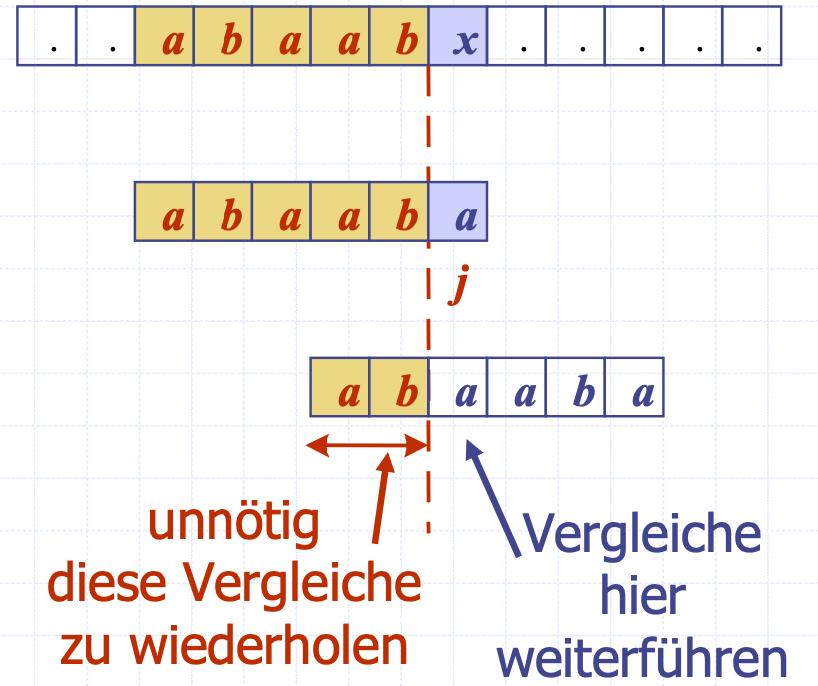
\includegraphics[scale=.2]{graphic/08 PatternMatching/KMP def.png}
\end{center}
\vspace{-8pt}
\subsubsection{Laufzeit}
\begin{itemize}
    \item failure function kann als Array dargestellt werden, in O(m) Zeit
\end{itemize}
\subsubsection{KMP Fehl-Funktion}
\begin{itemize}
    \item Vorlaufsphase sucht Algorithmus Übereinstimmungen von Präfixes des Musters im Muster selbst
    \item Die failure function F(j) ist definiert als die Grösse des längsten Präfixes von P[0..j] , so dass dieser auch Suffix von P[1..j] ist.
    \item KMP modifiziert den Brute-Force Algorithmus so, dass bei einer Differenz $P[j] \neq T[i]$ der Index j gesetzt wird mit: $ j \leftarrow F(j-1)$
\end{itemize}
\vspace{-8pt}
\begin{center}
    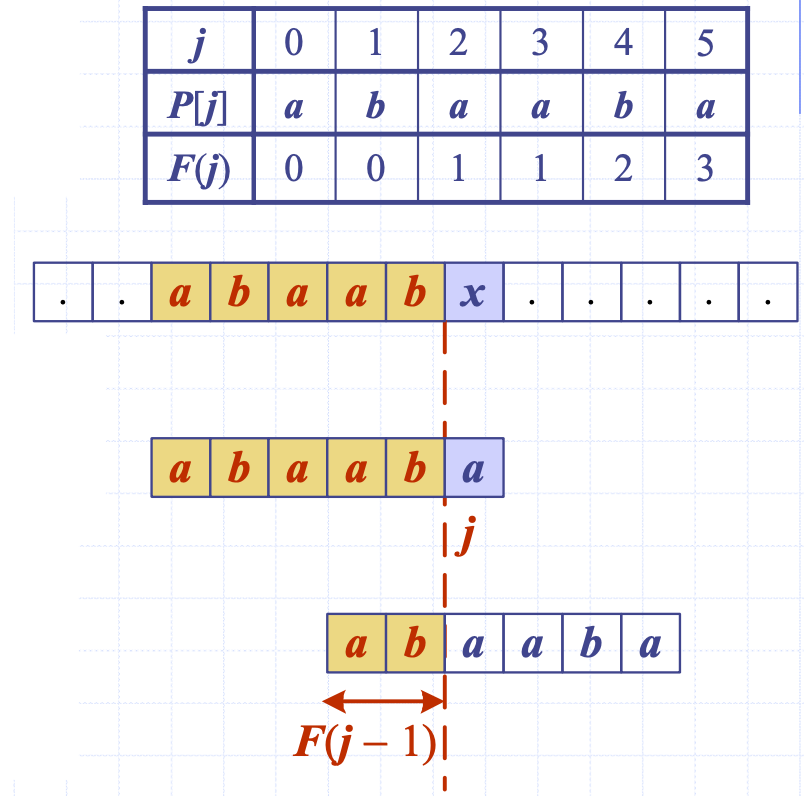
\includegraphics[scale=.2]{graphic/08 PatternMatching/KMP Fehl.png}
\end{center}
\vspace{-8pt}
\begin{lstlisting}
Algorithm failureFunction(P)
    F[0] <-- 0
    i <-- 1
    j <-- 0
    while i < m
        if P[i] == P[j]
        // we have matched j+1 chars
        F[i] <-- j+1
        i <-- i + 1
        j <-- j + 1
    else if j > 0
        // use failure function to shift P
        j <-- F[j-1]
    else
        F[i] <-- 0 // No match
        i <-- i + 1
\end{lstlisting}
\vspace{-8pt}
\begin{center}
    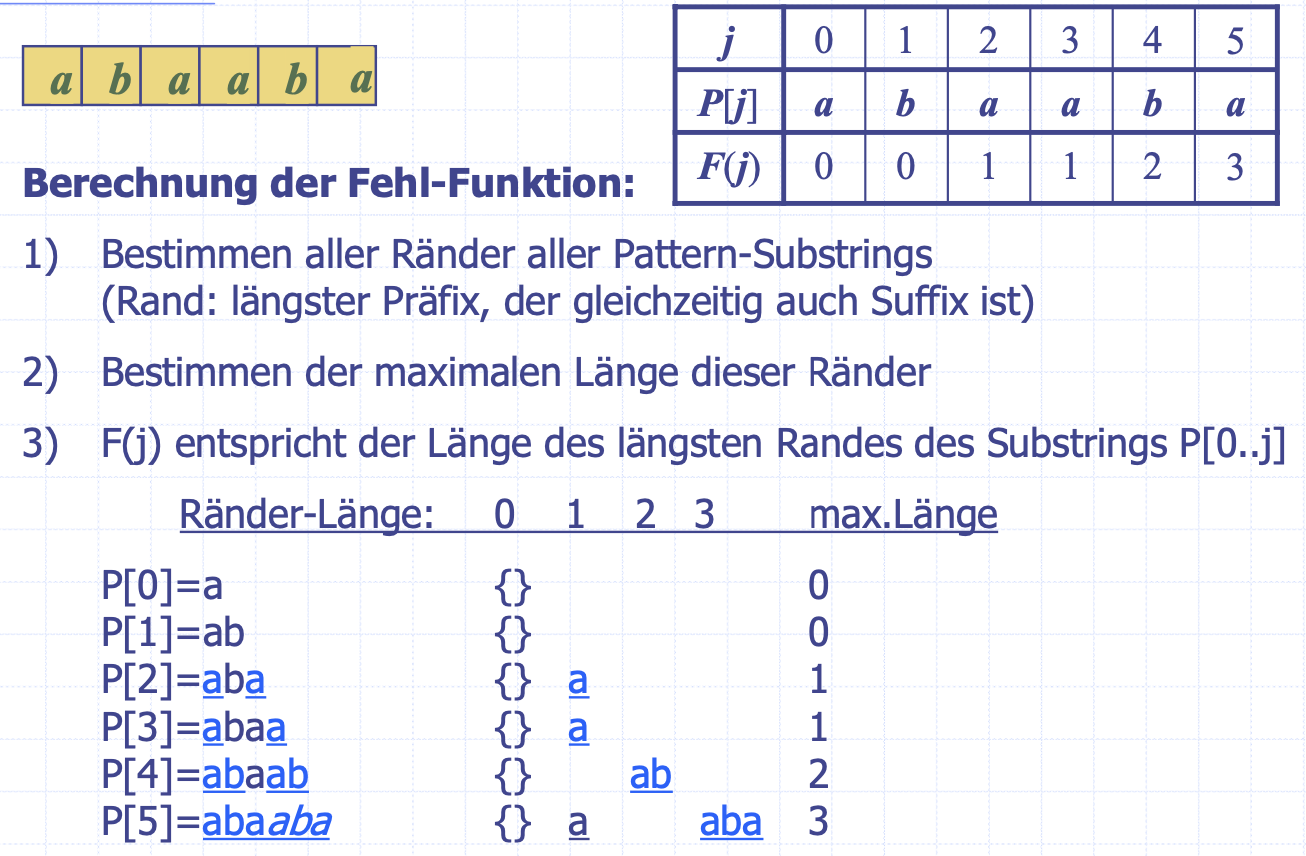
\includegraphics[scale=.25]{graphic/08 PatternMatching/KMP Fehl2.png}
\end{center}
\vspace{-8pt}

\subsubsection{Algorithmus}
Bei jeder Iteration der while- Schleife wird entweder:
\begin{itemize}
    \item i um eines erhöht
    \item Oder die Verschiebung i-j nimmt um mindestens 1 zu (F(j - 1) < j)
\end{itemize}
\begin{lstlisting}
Algorithm KMPMatch(T, P)
    F <-- failureFunction(P)
    i <-- 0
    j <-- 0
    while i < n
        if T[i] == P[j]
            if j == m -1
                return i - m + 1 // Match
            else
                i <-- i + 1
                j <-- j + 1
        else
            if j > 0
                j <-- F[j-1]
            else
                i <-- i + 1
    return -1 // No match
\end{lstlisting}
\vspace{-8pt}
\begin{center}
    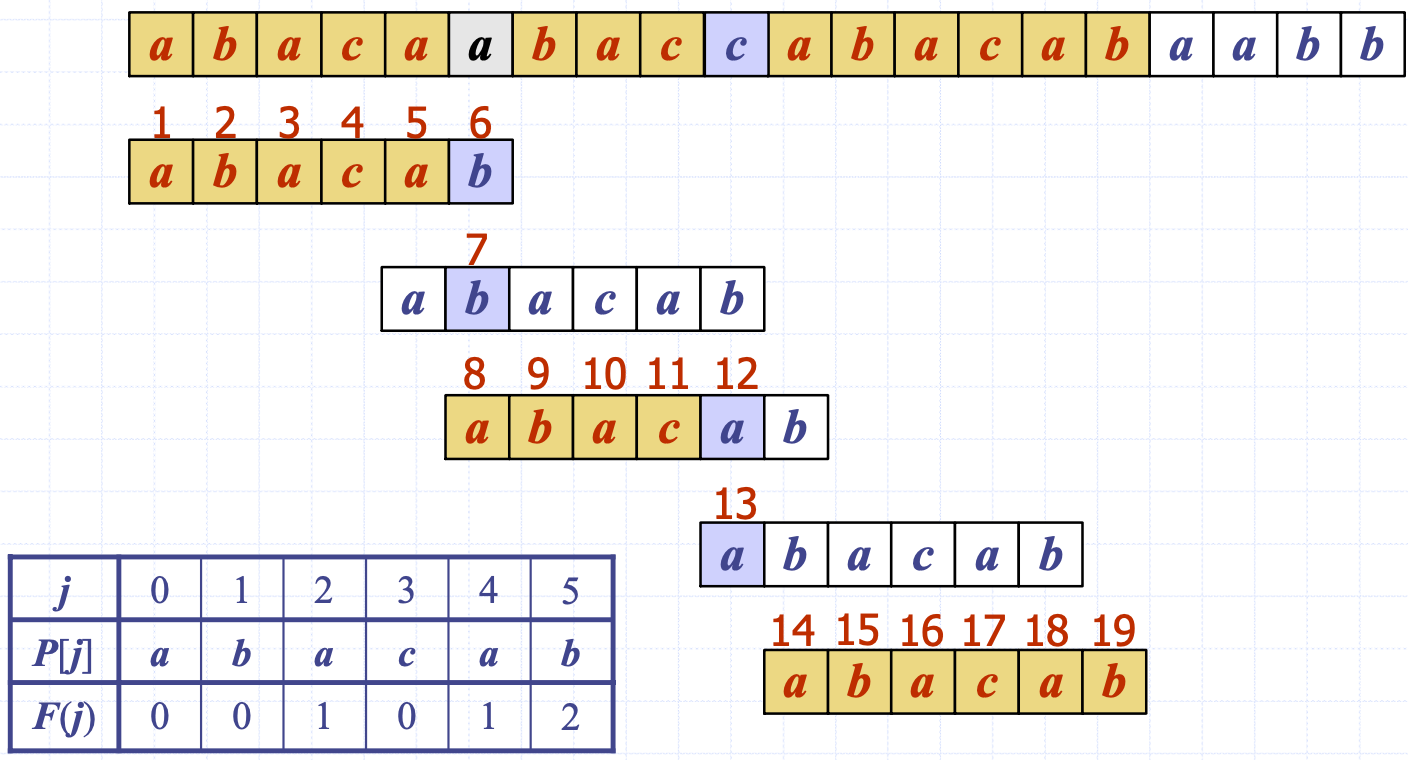
\includegraphics[scale=.2]{graphic/08 PatternMatching/KMP.png}
\end{center}
\vspace{-8pt}

\paragraph{Knuth-Morris-Pratt (KMP)}
\textbf{1. KMP Fehl-Funktion F(j) bestimmen}\\

\textbf{Spalte P(j):} Pattern selbst\\
\textbf{Spalte F(j):} Maximale Ränder Länge
\begin{center}
    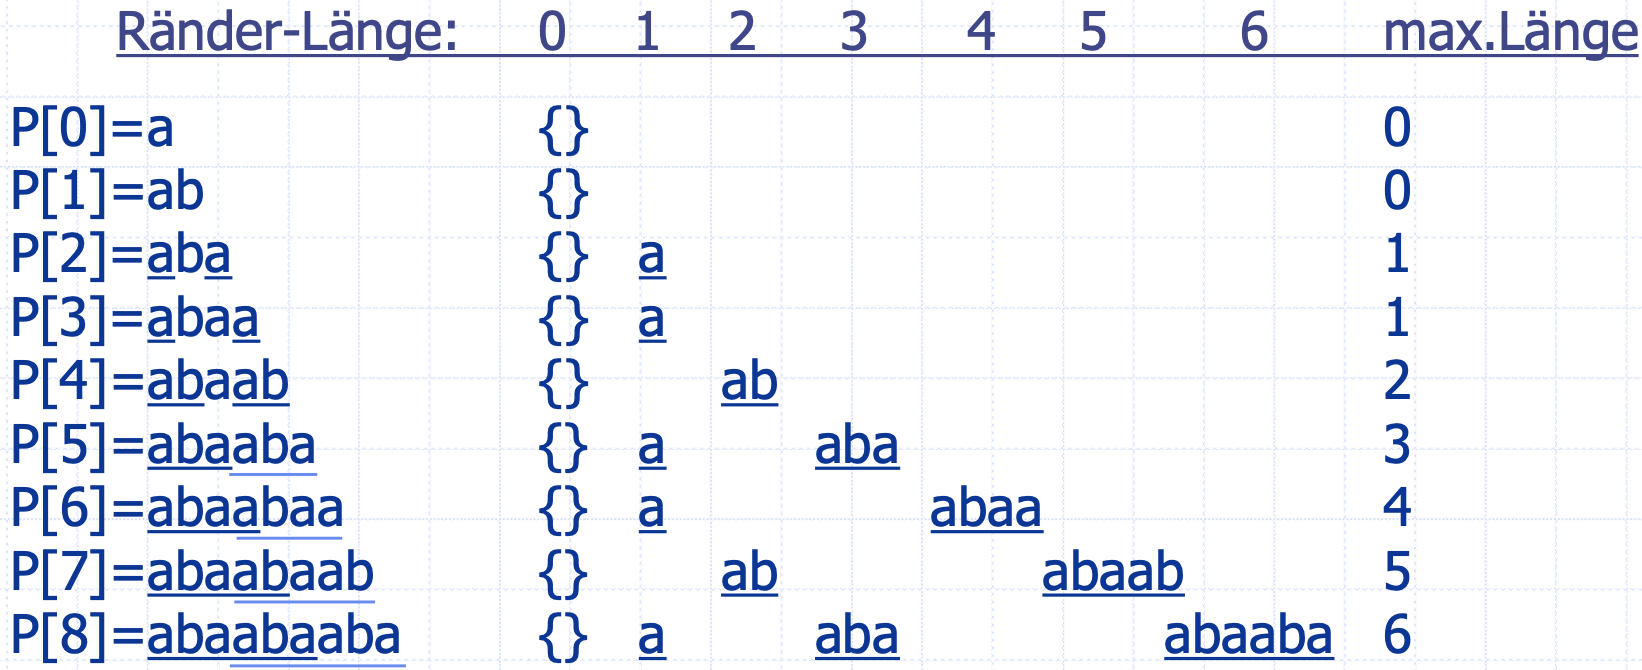
\includegraphics[scale=.2]{graphic/08 PatternMatching/KMP Fehl3.png}
\end{center}

\textbf{2. Vergleichen}\\
Immer der vordeste Buchstaben des Patterns wird mit Text verglichen!\\

\textbf{3. Missmatch}
\begin{center}
    \begin{tabular}[]{p{2cm} p{4cm}}
        Fehler ist 1. Buchstabe        & Verschiebung um 1 nach rechts\\
        \hline
         Fehler ist \underline{nicht} 1. Buchstabe & Fehlgeschlagener (Pattern-) Buchstabe im F(j) suchen\\
                & An Position F(j-1) verschieben (direkt unten) 
    \end{tabular}
\end{center}

\vfill
$ $

\newpage